\documentclass[tikz,border=10pt]{standalone}
\usepackage{tikz}
\usetikzlibrary{shapes.geometric, arrows.meta, positioning}

\begin{document}
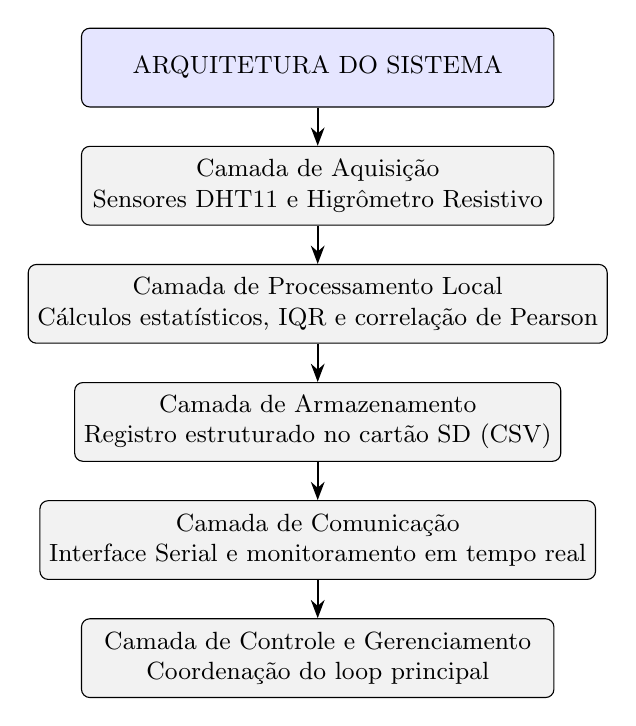
\begin{tikzpicture}[
    node distance=1.5cm,
    every node/.style={font=\small, align=center},
    box/.style={rectangle, draw=black, rounded corners=3pt, minimum width=6cm, minimum height=1cm, fill=gray!10},
    arrow/.style={-Stealth, thick}
]

% NODES
\node[box, fill=blue!10] (start) {ARQUITETURA DO SISTEMA};
\node[box, below of=start] (acquisition) {Camada de Aquisição\\Sensores DHT11 e Higrômetro Resistivo};
\node[box, below of=acquisition] (processing) {Camada de Processamento Local\\Cálculos estatísticos, IQR e correlação de Pearson};
\node[box, below of=processing] (storage) {Camada de Armazenamento\\Registro estruturado no cartão SD (CSV)};
\node[box, below of=storage] (communication) {Camada de Comunicação\\Interface Serial e monitoramento em tempo real};
\node[box, below of=communication] (control) {Camada de Controle e Gerenciamento\\Coordenação do loop principal};

% ARROWS
\draw[arrow] (start) -- (acquisition);
\draw[arrow] (acquisition) -- (processing);
\draw[arrow] (processing) -- (storage);
\draw[arrow] (storage) -- (communication);
\draw[arrow] (communication) -- (control);

\end{tikzpicture}
\end{document}

